\documentclass{article}
\usepackage[lmargin=3cm, tmargin=3cm, rmargin=2cm, bmargin=2cm]{geometry}
\usepackage[onehalfspacing]{setspace}
\usepackage[utf8]{inputenc}
\usepackage[T1]{fontenc}
\usepackage[brazil]{babel}
\usepackage{amsmath, bbm}
\usepackage{graphicx, graphics, xcolor, comment, enumerate, multirow, multicol, indentfirst}
\usepackage{hyperref}
\usepackage{float}
\usepackage{setspace} \doublespacing 

\title{MAP2212 - EP5 Estimativa de uma integral com base em geradores MCMC}
\author{Vinícius da Costa Collaço - 11811012 \and Nikolas Lukin - 5381328}

\renewcommand*\contentsname{Sumário}
\renewcommand\refname{Referências}

\begin{document}
\setlength{\parindent}{1cm} 
\maketitle
\begin{center}
\Large{Instituto de Matemática e Estatística}\\
\Large{Universidade de São Paulo}\\
\begin{figure}[htp]
  \centering
  
\includegraphics[scale=1]{Imagens/IME.jpg}
  \label{fig:IME}
\end{figure}
\Large{Junho de 2022}
\end{center}
\pagebreak
\tableofcontents
\pagebreak

\maketitle

\section{Introdução}
\indent
Esse relatório apresenta a solução do quinto exercício programa (EP5) proposto na matéria MAP2212/2022 (Laboratório de Computação e Simulação) do curso de bacharelado de matemática aplicada e computacional (BMAC) do instituito IME-USP. O objetivo deste EP é estimar a função verdade definida pela integral da distribuição de Dirichlet,

\begin{equation}
    W(v)= \int_{T(v)} f(\theta\mid x,y)d\theta 
\end{equation}

através de uma função aproximada \textit{U(v)} obtida pela integral condensada da massa de probabilidade\cite{kaplan1987improved} de $f(\theta|x,y)$ no domínio \textit {T(v)} e que não ultrapassa um nível \textit{v} pré-estabelecido (cut-off), ou seja,

\begin{equation}
    T(v)=\{ \theta  \in   \Theta  \mid f(\theta\mid x,y)\leq v\}
\end{equation}
\indent
A função \textit{f} é a função de densidade de probabilidade posterior de \textit{Dirichlet}, que representa um modelo estatístico m-dimensional multinomial, dado por:
\begin{equation}
    f(\theta\mid x,y) =  \frac{1}{B(x+y)}  \prod_{i=1}^m  \theta_i^{x_i+y_i-1} 
\end{equation}

onde \textit{x} é um vetor de observações, \textit{y} é um vetor de observações a priori, $\theta$ é um vetor simplex de probabilidades, \textit{m} = 3 é a dimensão e \textit{B} representa a distribuição Beta. Observe que, 

\begin{equation}
    x,y \in   \aleph ^m,  \theta  \in  \Theta =S_m=\{ \theta  \in  \Re _m^+ \mid f(\theta\mid x,y)\leq v\}
\end{equation}
\indent
Nas próximas seções demonstraremos como estimamos a função verdade usando integral condensada e a variante do Método de Monte Carlo de geradores randômicos usando Cadeias de Markov (MCMC), o qual é descrito a seguir. O algoritmo produzido utiliza a linguagem \textit{Python} e bibliotecas adequadas\cite{harris2020array, Waskom2021, Hunter:2007, 2020SciPy-NMeth}, 

\section{Estrutura do algoritmo de MCMC}
\indent
A idéia por trás do Método de Monte Carlo usando Cadeias de Markov é gerar amostras de pontos para o cálculo de uma integral em locais onde a função a ser integrada seja mais relevante. A localização destas amostras no domínio da função tendem a se convergir como em uma Cadeia de Markov. Inicialmente, algoritmo de MCMC cria amostras randômicas a partir de uma distribuição multivariada. Neste trabalho usamos a distribuição multivariada normal para gerar amostras de $\theta$ com média zero e matriz de variância definida por,

\begin{equation}
    Var(X_{i,j})=\left\{\begin{matrix}
\frac{\alpha _i(\alpha _0-\alpha _i)}{\alpha _0^2(\alpha _0+1)} & i=j\\ 
\frac{-\alpha _i\alpha _0}{\alpha _0^2(\alpha _0+1)} & i\neq j
\end{matrix}\right.
\end{equation}

onde, $\alpha _0=\sum_{i=1}^{k}\alpha _i$
\indent
Esse vetor é adicionado à um valor inicial de $\theta_i$ para tornar-se um candidato de amostra, o qual é validado pela verificação de pertencer ao domínio de um simplex:

\begin{itemize}
	\item Soma dos elementos do vetor é unitária
	\item Os elementos do vetor são estritamente positivos
\end{itemize}

\indent Caso as condições de domínio estejam satisfeitas, o algoritmo decide por aceitar ou rejeitar esse candidato ($\theta_{i+1}$com base no critério de balanço detalhado do algoritmo de Metrópolis-Hastings. Segundo este algoritmo, as amostras serão aceitas com base na probabilidade relativa na função a qual se deseja integrar. Ela será aceita caso um número aleatório uniforme em [0,1] seja menor que $\alpha(\theta_{i+1}, \theta_{i})$, o qual é definido por,

\begin{equation}
    \alpha(\theta_{i+1}, \theta_{i}) = min(1,\frac{f(\theta_{i+1}\mid x,y)}{f(\theta_{i}\mid x,y)}
\end{equation}
\indent
Caso contrário, $\theta_{i+1}$ continuará com o valor de $\theta_{i}$. Após gerados os \textit{n} valores da amostra, inicia-se o calculo da função potencial $p(\theta_i\mid x,y)$ correspondente à cada amostra,

\begin{equation}
    p(\theta\mid x,y) =  \prod_{i=1}^m  \theta_i^{x_i+y_i-1} 
\end{equation}
\indent
Finalmente a lista de potenciais gerados para cada amostra é ordenada e normalizada pela função Gamma. Esta lista é condensada em uma lista menor com \textit{k} bins, os quais cada um condensa a informação de \textit{n/k} pontos. Finalmente, o algoritmo percorre esta última lista e localiza a posição \textit{i} correspondente ao cut-off \textit{v} imposto na entrada. O valor calculado da integral condensada \textit{U(v)} é obtido por,

\begin{equation}
    \left\{\begin{matrix}
    U(v)= 0, & v \leq min(f(\theta\mid x,y))\\ 
    U(v)= \frac{i}{n} & min(f(\theta\mid x,y)) \leq v \leq max(f(\theta\mid x,y))\\ 
    U(v)= 1, & v \geq max(f(\theta\mid x,y))
    \end{matrix}\right.
\end{equation}
\indent
Resumidamente, o algoritmo está estruturado nas seguintes funções:

\begin{itemize}
	\item Declaração de variáveis e estruturação de objetos
	\item Cálculo da matriz de covariância
	\item Gerador de amostras
	\item Cálculo da função potencial das amostras
	\item Ordenação e normalização da lista
	\item Condensação da lista em bins
	\item Cálculo da probabilidade acumulada para um dado $v$
\end{itemize}

\subsection{Definindo o valor inicial e de aquecimento da cadeia}

Para valor inicial utilizou-se o valor central do simplex, ou seja, o vetor [1/3, 1/3, 1/3] e para aquecimento da cadeia é necessário o descarte das amostras iniciais, observou-se empiricamente que com uma queima de 1000 valores a cadeia se comportava como o esperado, definindo então 1000 como valor de queima.

\section{Definindo a quantidade de iterações n}
\indent
Utilizamos o mesmo método de cálculo da quantidade de pontos \textit{n} que serão utilizados na simulação que no EP4. Para tanto, considera-se a aproximação assintótica de uma distribuição Bernoulli para determinar a quantidade de pontos dentro de um bin necessários para satisfazer a resolução e o erro máximo tolerável.

\subsection{Erro $(\varepsilon)$}
\indent
Define-se por erro $(\varepsilon)$ a precisão esperada do cálculo, ou seja, o maior desvio tolerável entre o valor obtido por aproximação $U(v)$ e o valor exato da função verdade $W(v)$. Neste trabalho, foi considerado $\varepsilon = 0,0005$

\subsection{Número de bins (k)}
\indent
Para efeitos práticos os dados da simulação são condensados em bins\cite{kaplan1987improved}. A quantidade \textit{k} de bins da distribuição discreta de probabilidades deve ser tal a garantir uma resolução que seja maior que o erro $\epsilon$, definido em \ref{eqn:valork}

\begin{equation}
    W(v_j) - W(v_{j-1}) = \frac{1}{k} \geq \epsilon
    \label{eqn:valork}
\end{equation}

Portanto, para que a resolução seja maior que o erro estipulado, 

\begin{equation}
    k \geq \frac{1}{\epsilon} \implies k \geq 2000
    \label{eqn:valork}
\end{equation}

Para melhorar a resolução, considerou-se utilizar o dobro do mínimo de bins necessários, ou seja,

\begin{equation*}
    k = 4000
\end{equation*}

\subsection{Distribuição dos dados na amostra}

\indent Inicialmente, supõe-se que os dados estão distribuídos segundo uma distribuição de Bernoulli dentro dos bins. No entanto, caso o tamanho da amostra seja suficientemente grande, pelo teorema do limite central podemos aproximar esta Bernoulli por uma normal, obtendo:

\[
P(|\hat{p} - p|\leq \varepsilon)\geq \gamma 
\] \cite{estatbas}

\[
P(-\varepsilon \leq \hat{p} - p \leq \varepsilon) = P\left( \frac{-\sqrt{n}\varepsilon}{\sigma} \leq Z \leq \frac{\sqrt{n}\varepsilon}{\sigma}\right) \approx \gamma
\]

\indent A estimativa para a quantidade total de pontos \textit{n} a serem simulados é portanto,

\begin{equation}
    n = \frac {\sigma^2 {Z_\gamma}^2} {\varepsilon^2}
    \label{eqn:valorn}
\end{equation}

\indent O resultado obtido em \ref{eqn:valorn} será utilizado para definir o número de pontos necessários para resultar no erro mínimo exigido. Na modelagem normal da distribuição de dados do problema, consideramos um intervalo de confiança $\gamma = 95\%$, escolhido arbitrariamente. Obtêm-se assim $Z_\gamma = 1,96$ para $N(0,1)$,

\subsection{Variância amostral}

\indent Para o cálculo da variância, considera-se que os pontos se distribuem segundo uma distribuição de Bernoulli dentro de um bin com probabilidade igual à resolução do bin ($= \frac{1}{k}$). Com o valor de $k = 4000$ variância é determinada por,

\begin{equation}
    \sigma^2 = \frac{\epsilon}{2} (1 - \frac{\epsilon}{2}) \approx \frac{\epsilon}{2}
    \label{eqn:valorsig}
\end{equation}

\subsection{Valor final do n}
\indent
O valor de \textit{n} é obtido através das equações em \ref{eqn:valork} \ref{eqn:valorn} \ref{eqn:valorsig} resultando em,

\begin{equation*}
    n = k \cdot \frac{1,96^2\cdot \frac{\epsilon}{2}}{\epsilon^2} \geq 15.366.400
\end{equation*}

Porém observando os valores extremos dentro de um único bin empiricamente, observou-se que não havia diferença significante reduzindo em cerca de 10 vezes o tamanho da amostra.
Então optou-se por reduzir amostra final cerca de 7 vezes, para aumentar a eficiência do código e ainda assim manter uma boa acurácia, obtendo no final.

\[
    n_{final} = 2.000.000 \ pontos
\]

\section{Resultados e discussão}

\indent Para a simulação construiu-se um algoritmo que recebe como dados de entrada os vetores \textit{x} e \textit{y}, constrói e ordena uma lista com \textit{n} entradas crescentes de $f(\theta|x,y)$ obtidas de simulações aleatórias de $\theta_i$ advindas de um gerador gerador baseado no MCMC como descrito anteriormente. Verificou-se que o algoritmo funcionou conforme o esperado, apesar de demorar mais para rodar que o anterior. Uma comparação dos resultados do algoritmo do EP4 com este algoritmo está mostrada a seguir para validação dos resultados desta simulação com $x = [4,6,4]$ e $y = [1,2,3]$.

\begin{table}[h!]
\centering
 \begin{tabular}{||c c c||} 
 \hline
 v & U(v) EP4 & U(v) EP5 \\ [0.5ex] 
 \hline\hline
0 & 0.00000 & 0.00000 \\
1 & 0.04125 & 0.03700 \\
2 & 0.09050 & 0.08300 \\
3 & 0.14325 & 0.13450 \\
4 & 0.19875 & 0.18875 \\
5 & 0.25575 & 0.24575 \\
6 & 0.31450 & 0.30425 \\
7 & 0.37475 & 0.36450 \\
8 & 0.43625 & 0.42600 \\
9 & 0.49875 & 0.48900 \\
10 & 0.56200 & 0.55350 \\
11 & 0.62625 & 0.61850 \\
12 & 0.69150 & 0.68475 \\
13 & 0.75725 & 0.75150 \\
14 & 0.82375 & 0.81925 \\
15 & 0.89100 & 0.88800 \\
16 & 0.95875 & 0.95750 \\
17 & 1.00000 & 1.00000 \\ [1ex]
 \hline
 \end{tabular}
 \caption{Validação de \textit{U(v)}}
 \label{tab:validation}
\end{table}

\indent A comparação dos gráficos resultante de \textit{U(v)} de ambos EP4 e EP5 está ilustrada na Figura \ref{fig:int}:

\begin{figure}[htp]
  \centering
  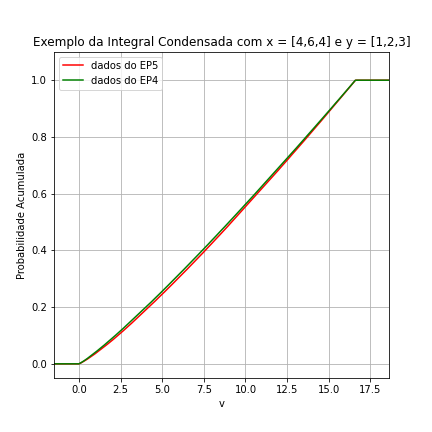
\includegraphics[scale=0.85]{Imagens/Integral.png}
  \caption{Gráfico de \textit{U(v)}}
  \label{fig:int}
\end{figure}

\section{Conclusão}

\indent A integral da distribuição de \textit{Dirichlet} foi calculada simulando-se pontos obtidos através de um gerador randômico baseado em Cadeias de Markov. O algoritmo foi implementado em Python e mostrou-se eficiente para cálculos de diversos \textit{U(v)} após a implementação da classe, cumprindo assim os requisitos exigidos pelo problema proposto. Além de se observar a convergência do resultado numérico, os mesmos foram coerentes com uma simulação fornecida pelo algoritmo anterior (EP4), o qual serviu de validação do método.

\newpage
\bibliographystyle{plain}
\bibliography{ref.bib}

\end{document}
